\begin{frame}
    \frametitle{Transition analysis}
    To meet the first objective, I model the transition from the current 
    \gls{LWR} fleet to advanced reactors
    \begin{itemize}
        \item Use fuel cycle simulators to model the transition
        \item Model the deployment and decommissioning of fuel cycle facilities 
        \item Model material transactions between facilities
        \item Quantify material requirements to understand potential \gls{HALEU}
              demand
    \end{itemize}

\end{frame}

\begin{frame}
    \frametitle{Transition analysis assumptions}
    \begin{columns}
        
    \column[t]{6cm}
    \vspace{-0.9cm}
    \begin{figure}
    \centering
    \begin{tikzpicture}[node distance=1.5cm]
        \node (mine) [facility] {Uranium Mine};
        \node (enrichment) [facility, below of=mine]{Enrichment};
        \node (reactor) [facility, below of=enrichment]{Reactor};
        \node (adv_reactor) [transition, right of=reactor, xshift=3cm]{Advanced Reactor};
        \node (wetstorage) [facility, below of=reactor]{Cooling Pool};
        %\node (drystorage) [facility, below of=wetstorage]{Dry Storage};
        \node (cooling) [transition, below of=adv_reactor]{Cooling Pool};
        \node (sinkhlw) [facility, below of=wetstorage, xshift=2.5cm]{HLW Sink};
        \node (sinkllw) [facility, left of=enrichment, xshift=-3cm]{LLW Sink};

        \draw [arrow] (mine) -- node[anchor=east]{Natural U} (enrichment);  
        \draw [arrow] (enrichment) -- node[anchor=south]{Tails}(sinkllw);
        \draw [arrow] (enrichment) -- node[anchor=east]{Fresh UOX}(reactor);
        \draw [arrow] (enrichment) -| node[anchor=west]{Fresh HALEU and LEU}(adv_reactor);
        \draw [arrow] (reactor) -- node[anchor=east]{Spent UOX}(wetstorage);
        \draw [arrow] (wetstorage) |- node[anchor=east]{Cool Spent UOX}(sinkhlw);
        %\draw [arrow] (drystorage) |- node[anchor=east]{Casked Spent UOX}(sinkhlw);
        \draw [arrow] (adv_reactor) -- node[anchor=west]{Spent Fuel}(cooling);
        \draw [arrow] (cooling) |- node[anchor=west]{Cooled Spent HALEU and LEU}(sinkhlw);`'

        \end{tikzpicture}
    \caption{Fuel cycle facilities and material flow between facilities in the 
    once-through fuel cycles modeled. Facilities in 
    blue are used in all once-through scenarios, the facilities in red are added in
    at the transition start time in the transition scenarios.}
    \label{fig:once-through_fuel_cycle}
\end{figure}

        \column[t]{4.5cm}
        Model transitions using \Cyclus \cite{huff_fundamental_2016}
        \begin{itemize}
            \item Simulations model reactor deployment from 1965-2090
            \item Transitions begin in 2025
            \item<2-> \gls{LWR} commission dates are obtained from the IAEA PRIS
                database \cite{noauthor_power_1989}
            \item<2-> \glspl{LWR} are assumed to operate until their current license 
                expires
            \item<3-> Manually calculate advanced reactor deployment
            \item<3-> Assume natural uranium is enriched to produce all 
                  fuel
        \end{itemize}

\end{columns}
\end{frame}

\begin{frame}
    \frametitle{Advanced reactors}
    \vspace{-0.2cm}
    \begingroup
        \renewcommand{\arraystretch}{1.5}
        \begin{table}
            \small
            \caption{Advanced reactor design specifications}
            \label{tab:reactor_summary}
            \vspace{-0.15cm}
            \begin{tabular}{ l p{1.5cm} p{1.5cm} p{2cm} }
                \hline
                Design Criteria & USNC MMR 
                    \cite{noauthor_usnc_2021} & 
                    X-energy Xe-100 \cite{mulder_overview_2021} & 
                    NuScale VOYGR \cite{nuscale_chapter_2020-1,reyes_nuscale_2021,reyes_correction_2022}\\\hline
                Reactor type & HTGR & HTGR & SMR\\
                Fuel type & UO$_2$ FCM & UCO TRISO & UO$_2$ pellets \\
                Power (MWe) & 5 & 80 & 77\\
                Power (MWth) & 15 & 200 & 250\\
                Enrichment (\% $^{235}U$) & 19.75 & 15.5 & 4.09 \\
                Cycle Length (yr) & 20 & Online & 1.5 \\
                Number of cycles & 1 & 6 & 3\\
                Reactor Lifetime (yr) & 20 & 60 & 60\\
                Burnup ($\frac{MWd}{kg U}$) & 82 & 168 & 45\\
                \hline
            \end{tabular}
        \end{table}   
    \endgroup
    \begin{equation}
        \text{mass (kg)} = \frac{\text{Power (MWth) * cycle length (d)*number of cycles}}{\text{Burnup (MWd/kg)}}
        \label{eq:fuel_mass}
    \end{equation}
\end{frame}

\begin{frame}
    \frametitle{Once-through scenario definitions}
        \begin{table}[ht]
            \centering
            \caption{Summary of the once-through fuel cycle transition scenarios.
                     Energy growth is relative to energy from \glspl{LWR} in 2025.}
            \label{tab:scenarios_once-through}
            \begin{tabular}{c l l}
                    \hline
                    Scenario number & Reactors present & Energy demand\\\hline
                    \rowcolor{lightblue} 1 & \glspl{LWR} & N/A \\
                    \rowcolor{lightorange}2 & \glspl{LWR} and MMR & No growth \\
                    \rowcolor{lightorange}3 & \glspl{LWR} and Xe-100 & No growth \\
                    \rowcolor{lightorange}4 & \glspl{LWR}, Xe-100, and MMR& No growth\\
                    \rowcolor{lightorange}5 & \glspl{LWR}, MMR, and VOYGR & No growth\\
                    \rowcolor{lightorange}6 & \glspl{LWR}, Xe-100, and VOYGR & No growth\\
                    \rowcolor{lightorange}7 & \glspl{LWR}, Xe-100, MMR, and VOYGR & No growth\\
                    \rowcolor{lightpink}8 & \glspl{LWR} and MMR& 1\% growth \\
                    \rowcolor{lightpink}9 & \glspl{LWR} and Xe-100 & 1\% growth\\
                    \rowcolor{lightpink}10 & \glspl{LWR}, Xe-100, and MMR& 1\% growth\\
                    \rowcolor{lightpink}11 & \glspl{LWR}, MMR, and VOYGR & 1\% growth\\
                    \rowcolor{lightpink}12 & \glspl{LWR}, Xe-100, and VOYGR & 1\% growth\\
                    \rowcolor{lightpink}13 & \glspl{LWR}, Xe-100, MMR, and VOYGR & 1\% growth\\
                    \hline
            \end{tabular}
        \end{table}
        %<2-> \tikz[overlay, remember picture]{\draw{draw=red,thick, double, fillopacity=0.2] ($(infrastructure)+(-0.5,0.4)$) rectangle ($(infrastructure)+(6,-0.2)$);}} 
\end{frame}

\begin{frame}
    \frametitle{Once-through scenario definitions}
        \begin{table}[ht]
            \centering
            \caption{Summary of the once-through fuel cycle transition scenarios.
            Energy growth is relative to energy from \glspl{LWR} in 2025.}
            \label{tab:scenarios_once-through}
            \begin{tabular}{c l l}
                \hline
                Scenario number & Reactors present & Energy demand\\\hline
                \rowcolor{lightblue} 1 & \glspl{LWR} & N/A \\
                \rowcolor{lightorange}\marktopleft{a3}2 & \glspl{LWR} and MMR & No growth \\
                \rowcolor{lightorange}3 & \glspl{LWR} and Xe-100 & No growth \\
                \rowcolor{lightorange}4 & \glspl{LWR}, Xe-100, and MMR& No growth\\
                \rowcolor{lightorange}5 & \glspl{LWR}, MMR, and VOYGR & No growth\\
                \rowcolor{lightorange}6 & \glspl{LWR}, Xe-100, and VOYGR & No growth\\
                \rowcolor{lightorange}7 & \glspl{LWR}, Xe-100, MMR, and VOYGR & No growth
                \markbottomright{a3}\\
                \rowcolor{lightpink}8 & \glspl{LWR} and MMR& 1\% growth \\
                \rowcolor{lightpink}9 & \glspl{LWR} and Xe-100 & 1\% growth\\
                \rowcolor{lightpink}10 & \glspl{LWR}, Xe-100, and MMR& 1\% growth\\
                \rowcolor{lightpink}11 & \glspl{LWR}, MMR, and VOYGR & 1\% growth\\
                \rowcolor{lightpink}12 & \glspl{LWR}, Xe-100, and VOYGR & 1\% growth\\
                \rowcolor{lightpink}13 & \glspl{LWR}, Xe-100, MMR, and VOYGR & 1\% growth\\
                \hline
        \end{tabular}
        \end{table}
        %<2-> \tikz[overlay, remember picture]{\draw{draw=red,thick, double, fillopacity=0.2] ($(infrastructure)+(-0.5,0.4)$) rectangle ($(infrastructure)+(6,-0.2)$);}} 
\end{frame}

\begin{frame}
    \frametitle{Advanced reactor deployment scheme}
    \begin{columns}
        \column[t]{5cm}
            Manually calculate the deployment scheme for advanced reactors
            \begin{itemize}
                \item Preferentially deploy reactors with larger power output first
                \item Deploy reactor with largest power output until an oversupply 
                      of power would be produced, deploy the next reactor until 
                      an oversupply of power, then deploy the last reactor until 
                      demand is met
                \item Deployment schedule is given to \Cyclus
            \end{itemize}
        \column[t]{5.5cm}
            \begin{figure}
                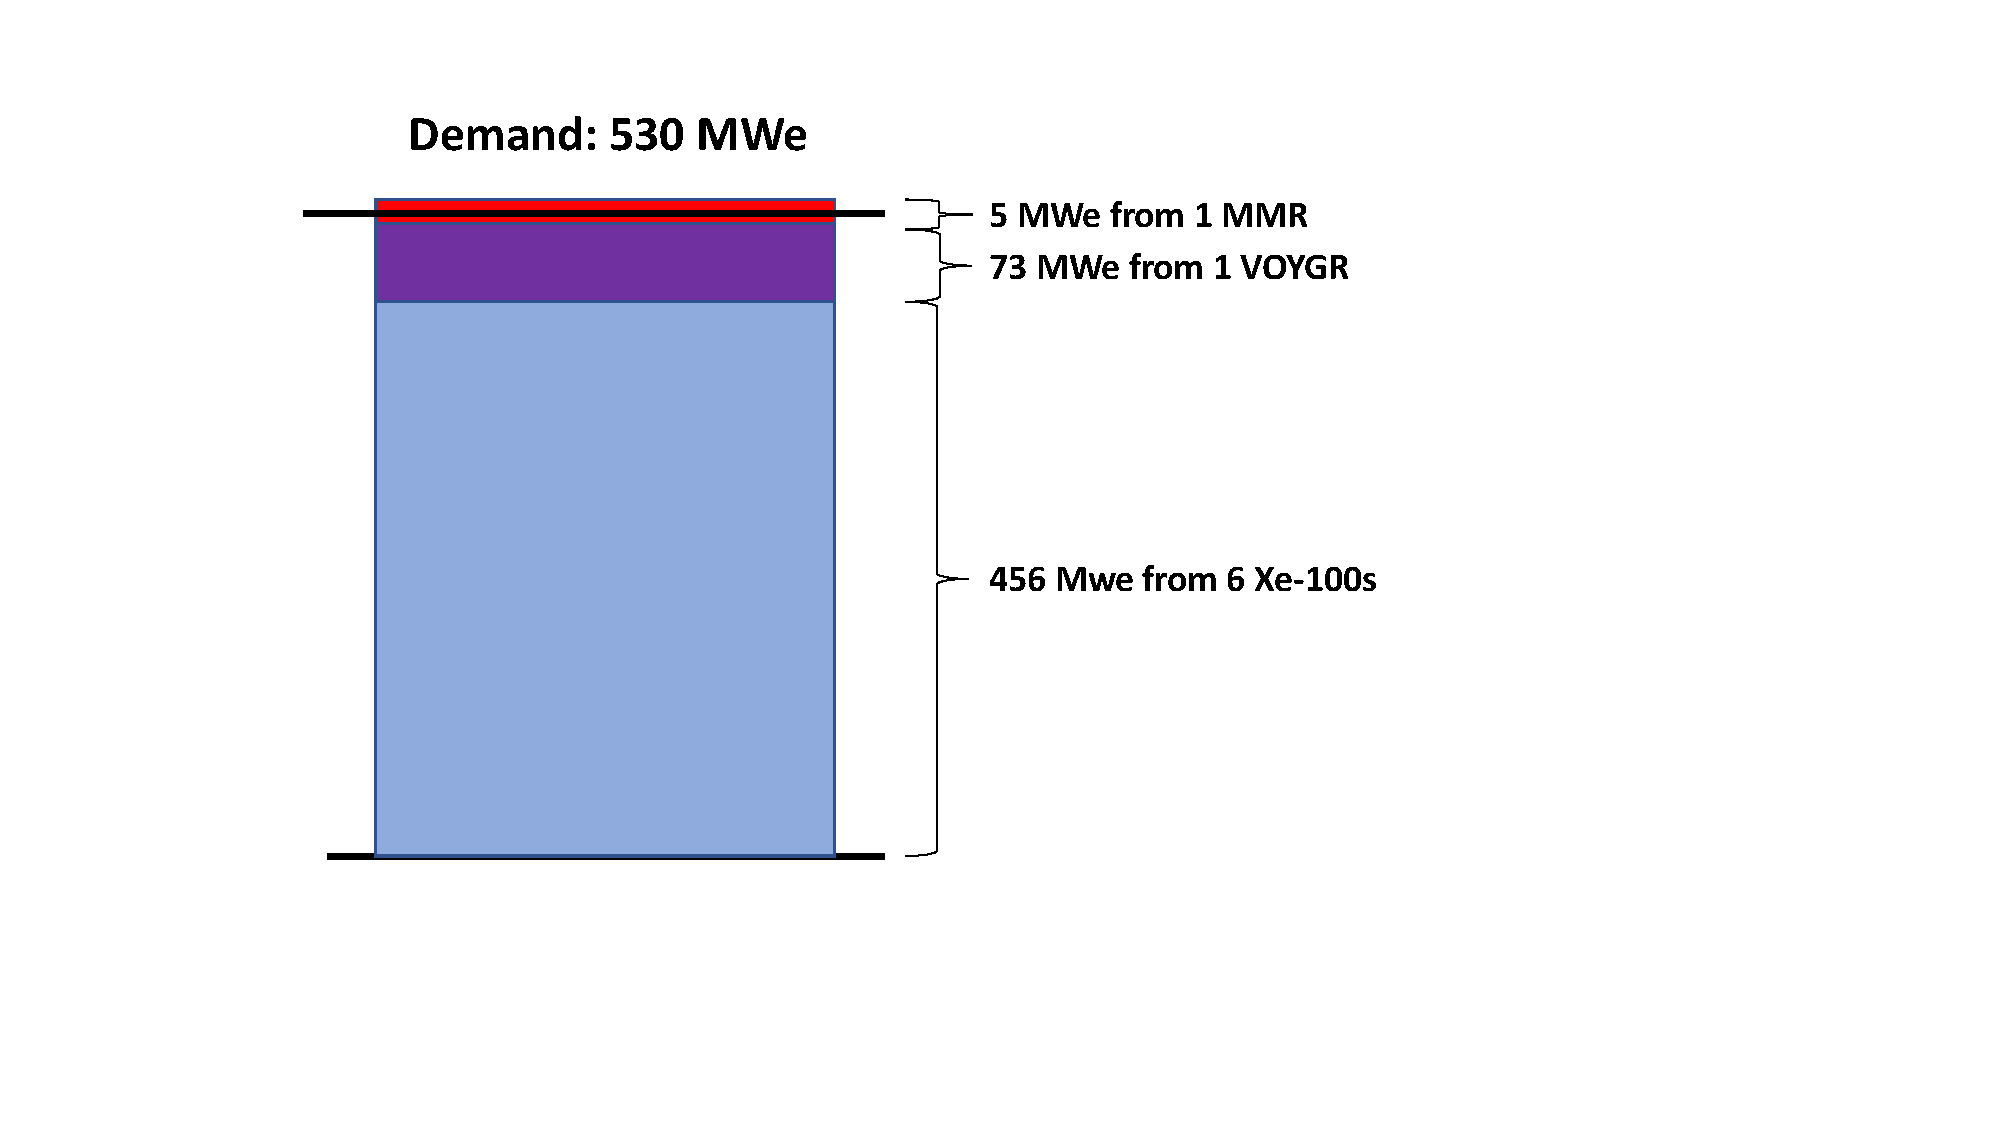
\includegraphics[scale=0.35, trim=200 100 50 50,clip]{Deployment_Scheme.pdf}
                \caption{Example of how advanced reactors in Scenario 7 are deployed to 
                meet a demand of 478 MWe.}
                \label{fig:deployment}
            \end{figure}
                    
    \end{columns}
\end{frame}